% chapter6_design.tex

\section{Chapter Overview}
This chapter presents the complete architectural and detailed design of \textbf{RootLens}. Beginning with the overall system architecture, it proceeds through the component-level design of each major subsystem, data flow diagrams, sequence diagrams, database design, and API design, concluding with key design decisions and their justifications. Three aspects of the design represent \textbf{original contributions}: (1) the category-specific ML explainer routing pattern, where the rule-based engine's primary classification determines which specialised ML model is invoked, avoiding the complexity of a monolithic multi-class classifier; (2) the 60/40 hybrid confidence combination model, empirically calibrated to produce monotonically reliable scores; and (3) the graceful degradation architecture that preserves rule-based functionality when the ML service is unavailable, ensuring the system never produces a worse outcome than a purely deterministic approach.

\section{Design Goals}
The design goals for RootLens are derived from the non-functional requirements specified in Chapter~4. These attributes guide the design of every component and are maintained system-wide:

\begin{itemize}
    \item \textbf{Accuracy:} Root cause classification accuracy $\geq$ 95\% and sub-cause accuracy $\geq$ 80\% (NFR02, NFR03), achieved through the hybrid rule-ML architecture.
    \item \textbf{Performance:} End-to-end diagnostic latency under 300ms (NFR01), enabling real-time consumption by dashboards and alerting pipelines.
    \item \textbf{Reliability:} Graceful degradation to rule-based analysis when the ML service is unavailable, ensuring no diagnostic capability is lost.
    \item \textbf{Explainability:} Every diagnosis accompanied by confidence scores and feature importances, enabling engineers to critically evaluate outputs rather than accept them blindly.
    \item \textbf{Deployability:} Automated deployment via Kubernetes Operator with a single Custom Resource, minimising manual configuration.
    \item \textbf{Usability:} Dashboard interface presenting diagnostic results clearly to engineers at varying experience levels.
\end{itemize}

\section{Overall System Architecture}
The architecture addresses all four research questions: the data collection layer provides the timing signals for RQ1, the intelligence layer implements the classification and feature engineering for RQ1-RQ2, the confidence combination model addresses RQ3, and the full pipeline enables the baseline comparison for RQ4. RootLens is composed of five independently deployable components:

\begin{enumerate}
    \item \textbf{Data Collection Module:} Concurrent Go goroutines that watch the \textbf{Kubernetes} API, KEDA state, and RabbitMQ metrics, assembling structured observation records on detection of a scaling event.
    \item \textbf{Rule-Based RCA Engine:} A deterministic Go package applying threshold-based classification to timing snapshots, producing a root cause category and a rule-based \textbf{confidence score}.
    \item \textbf{ML Explainer Service:} A Python Flask application hosting three category-specific \textbf{Random Forest} models, returning sub-cause predictions, class probabilities, and \textbf{feature importance} vectors via HTTP POST.
    \item \textbf{Backend REST API:} A Go HTTP server exposing RCA results, history, statistics, and health endpoints.
    \item \textbf{React Dashboard:} A single-page application visualising RCA results, confidence trends, sub-cause distributions, and system health in real time.
\end{enumerate}

Figure \ref{fig:architecture} illustrates the four-layer architecture. The Intelligence Layer is the only layer involving cross-service HTTP communication.

\begin{figure}[H]
\centering
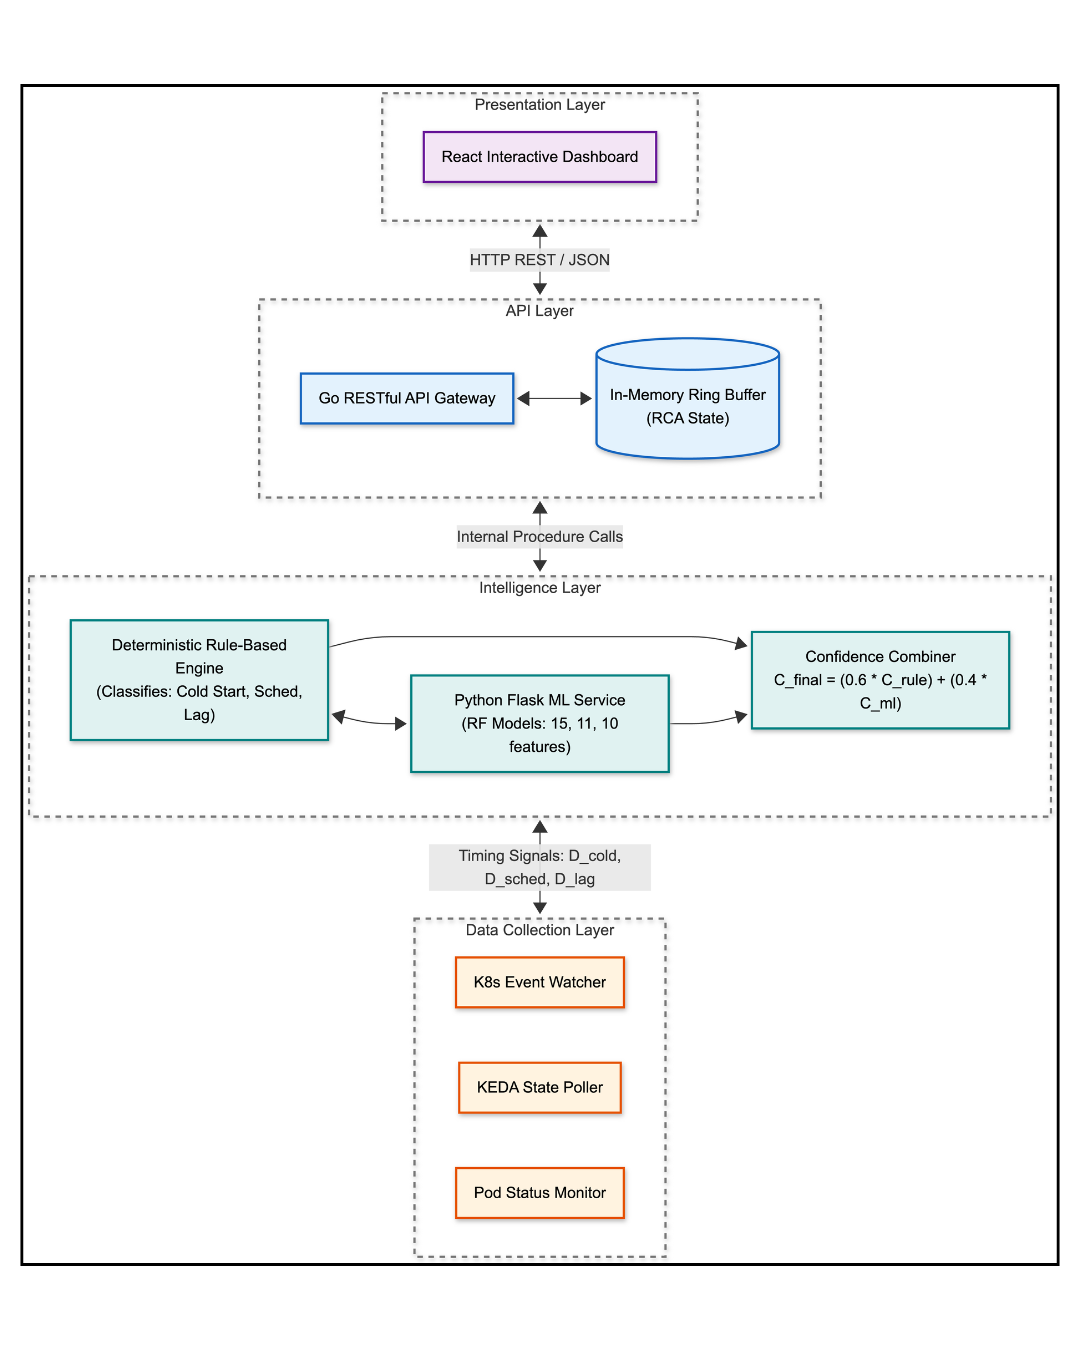
\includegraphics[width=0.85\textwidth]{thesis/assets/system_architecture.png}
\caption{RootLens System Architecture}
\label{fig:architecture}
\end{figure}

\section{Component-Level Design}

\subsection{Data Collection Module}
The data collection module comprises four concurrent components: a Kubernetes Event Watcher streaming pod lifecycle events via \texttt{client-go} Watch API, a KEDA State Poller checking ScaledObject replica changes every 5 seconds, a Pod Status Monitor computing scheduling and startup durations from phase transitions, and a RabbitMQ Metrics Collector capturing queue depth at KEDA trigger time.

\subsection{RCA Engine}
The rule-based RCA engine applies the following classification logic. Let $D_{cold}$, $D_{sched}$, and $D_{lag}$ be the three primary timing signals:

\begin{align}
D_{cold} &= t_{ready} - t_{pulling} \quad \text{(total container startup duration, seconds)} \\
D_{sched} &= t_{scheduled} - t_{created} \quad \text{(time from pod creation to node assignment, seconds)} \\
D_{lag} &= t_{keda\_trigger} - t_{queue\_event} \quad \text{(time from queue spike to KEDA reaction, seconds)}
\end{align}

Classification follows a priority-ordered decision tree:

\begin{enumerate}
    \item If $D_{cold} > 30s$ AND $D_{sched} < 5s$: classify as \texttt{ColdStart}
    \item If $D_{sched} > 10s$: classify as \texttt{Scheduling}
    \item If $D_{lag} > 45s$: classify as \texttt{MetricPropagation}
    \item Otherwise: classify as \texttt{Unknown}
\end{enumerate}

The rule-based confidence $C_{rule}$ is computed as:

\begin{equation}
C_{rule} = \min\left(1.0,\ \frac{\text{signal\_strength}}{\text{threshold}} \times 0.85\right)
\end{equation}

where signal\_strength is the magnitude of the dominant timing signal relative to its classification threshold, and 0.85 is a ceiling that reserves headroom for the ML contribution.

\subsection{ML Explainer Service}
The ML explainer service hosts three category-specific Random Forest classifiers. Table \ref{tab:ml_models} summarises each model.

\begin{table}[H]
\centering
\begin{tabularx}{\textwidth}{|l|l|l|X|}
\hline
\textbf{Model} & \textbf{Features} & \textbf{Samples} & \textbf{Sub-Cause Classes} \\ \hline
Cold Start Explainer & 15 & 42 train / 8 test & image\_pull\_latency, slow\_registry, readiness\_probe\_failure, init\_container\_delay, image\_pull\_backoff \\ \hline
Scheduling Explainer & 11 & 42 train / 8 test & cpu\_contention, memory\_pressure, node\_affinity\_mismatch, taint\_mismatch, resource\_quota\_exceeded \\ \hline
Metric Propagation Explainer & 10 & 34 train / 6 test & keda\_polling\_interval, queue\_depth\_spike, consumer\_processing\_lag, metric\_server\_delay \\ \hline
\end{tabularx}
\caption{ML Explainer Model Specifications}
\label{tab:ml_models}
\end{table}

Each model is served by a dedicated Flask route, returning the predicted sub-cause, class probabilities, and top-5 feature importances.

\subsection{Backend API}
The Go REST API provides CORS support, request logging, and error recovery middleware.

\subsection{Frontend Dashboard}
The React 19 dashboard provides five pages (Overview, Analysis, History, Trends, and Health) that visualise RCA results, confidence trends, sub-cause distributions, and component health status in real time.

\section{Data Flow Diagrams}
Figure \ref{fig:dfd} presents the Level 1 DFD, showing the transformation of raw observability signals into actionable diagnoses and the storage and retrieval paths through the in-memory ring buffer.

\begin{figure}[H]
\centering
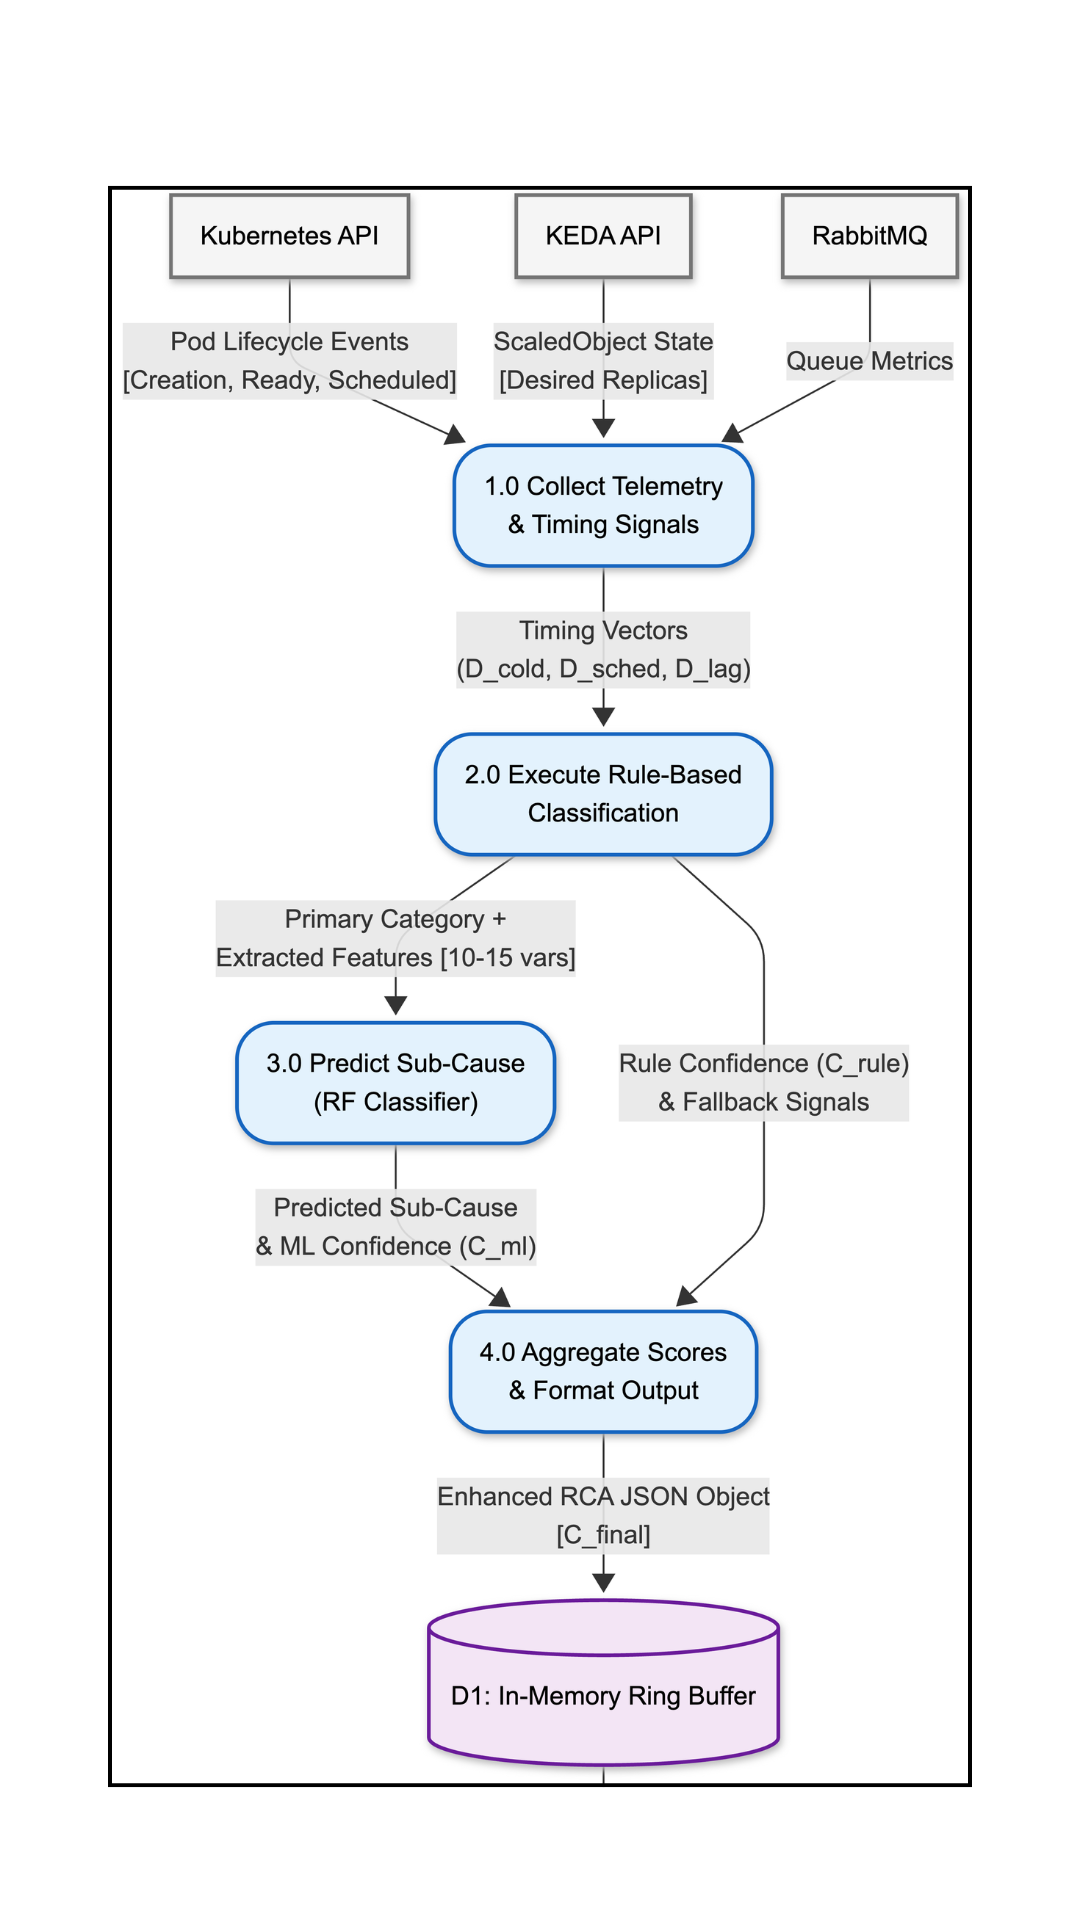
\includegraphics[width=0.55\textwidth]{thesis/assets/data_flow_diagram.png}
\caption{Level~1 Data Flow Diagram for RootLens Pipeline}
\label{fig:dfd}
\end{figure}

\section{Sequence Diagrams}
Figure \ref{fig:sequence} traces a single scaling event from the Kubernetes event stream to the rendered dashboard result, including the graceful degradation path when the ML Service is unreachable.

\begin{figure}[H]
\centering
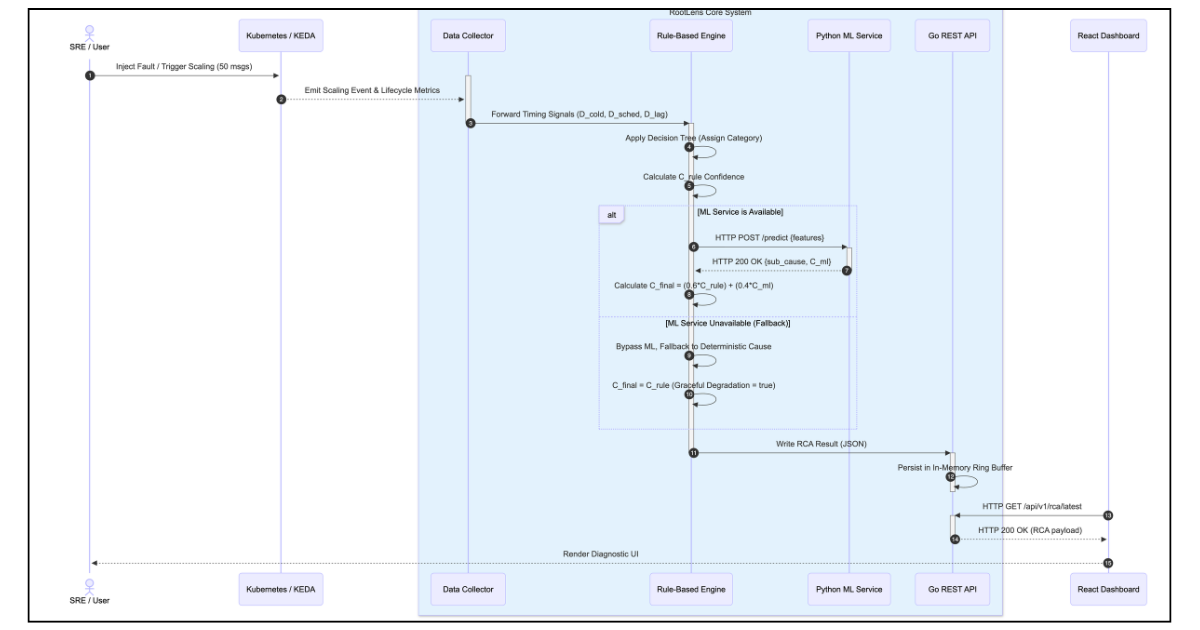
\includegraphics[width=0.85\textwidth]{thesis/assets/sequence_diagram.png}
\caption{Sequence Diagram for a Single RCA Event}
\label{fig:sequence}
\end{figure}

\section{Component Diagram}
Figure \ref{fig:component} presents the three principal software components using UML component notation, exposing internal package structure and inter-component dependencies.

\begin{figure}[H]
\centering
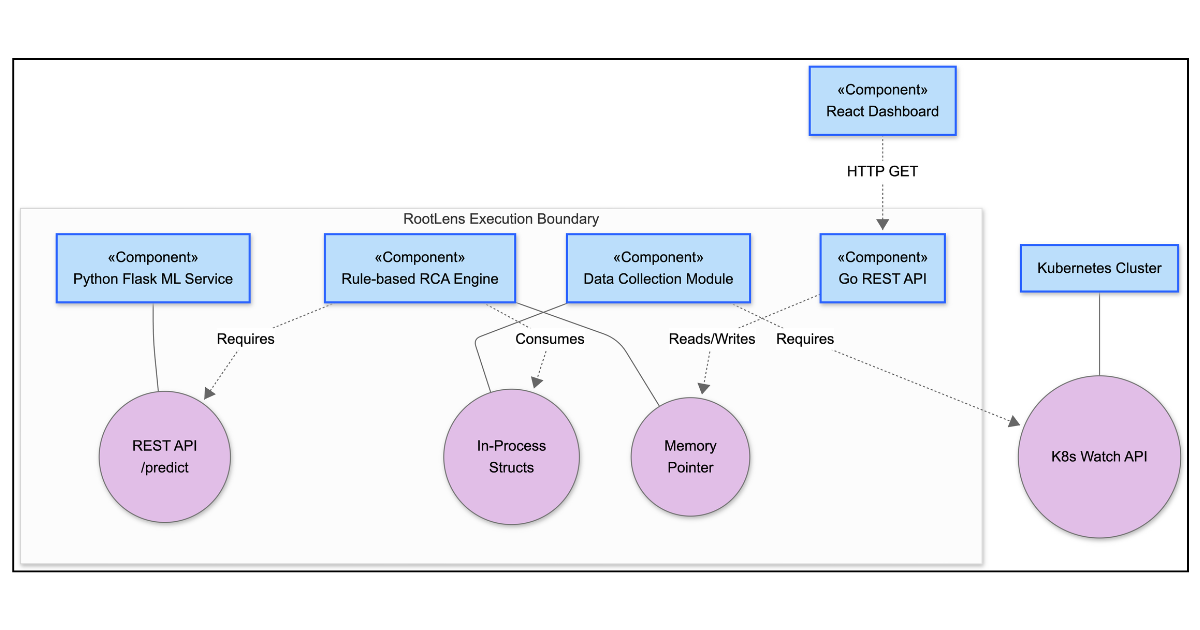
\includegraphics[width=0.85\textwidth]{thesis/assets/component_diagram.png}
\caption{Component Diagram of RootLens system}
\label{fig:component}
\end{figure}

\section{Deployment Diagram}
Figure \ref{fig:deployment} shows the two supported deployment configurations: Docker Compose for development and the kubebuilder v4 Operator for Kubernetes cluster deployments.

\begin{figure}[H]
\centering
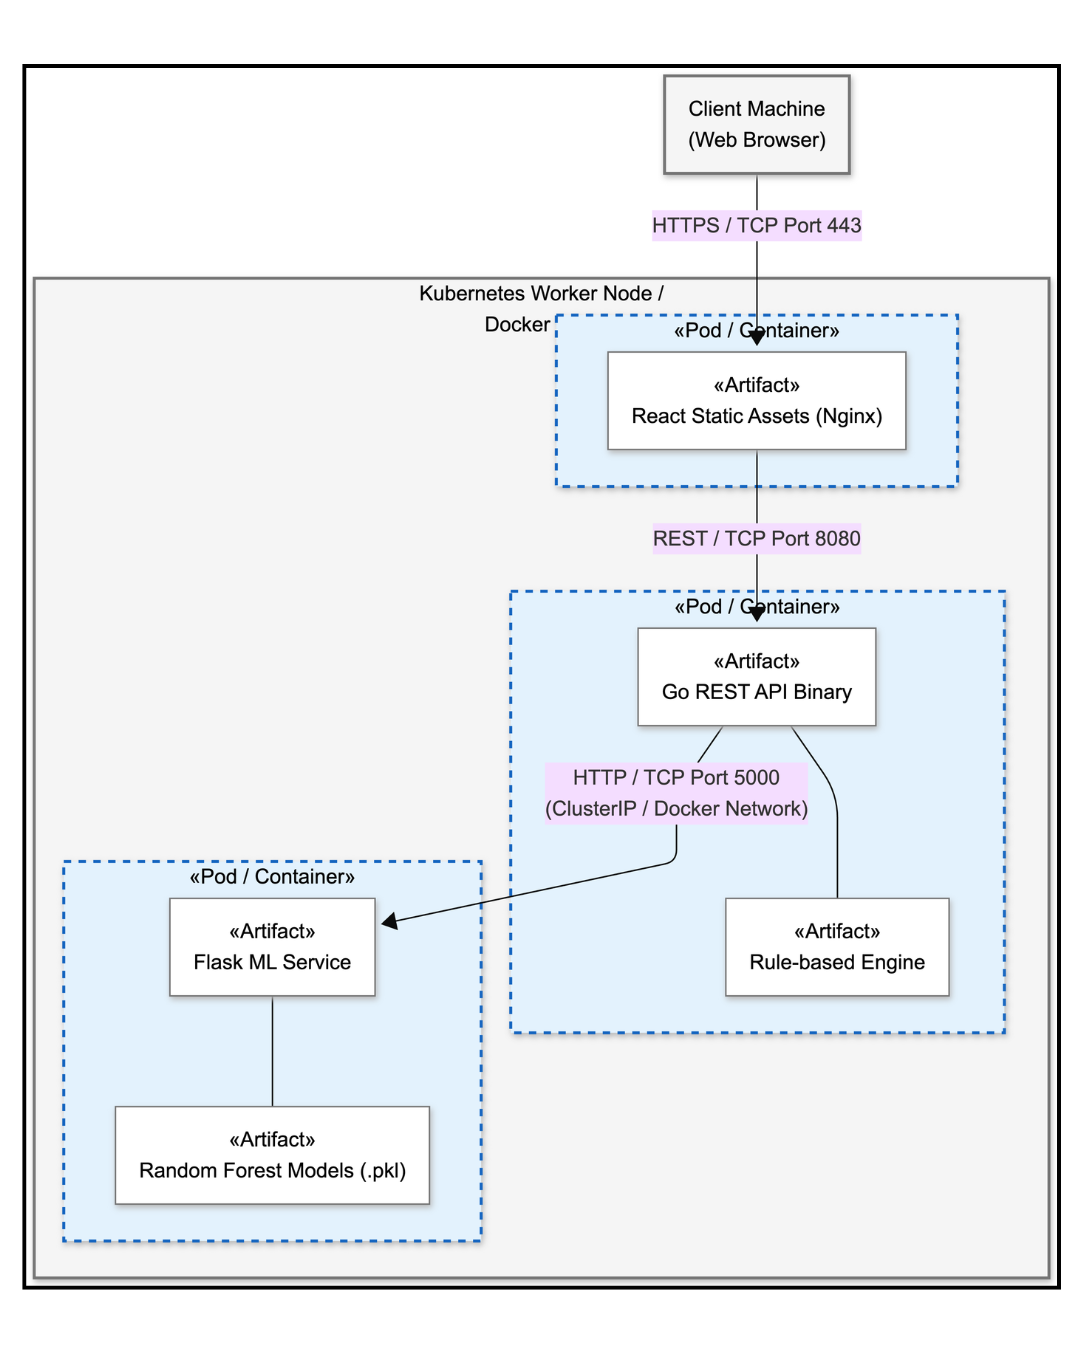
\includegraphics[width=0.85\textwidth]{thesis/assets/deployment_diagram.png}
\caption{Deployment Diagram: Docker Compose (development) and Kubernetes (production)}
\label{fig:deployment}
\end{figure}

\section{Database / Data Storage Design}
RootLens uses an in-memory \textbf{ring buffer} as its primary data store for RCA results. It is implemented as a fixed-capacity slice of 50 EnhancedRCAResult structs protected by a sync.RWMutex, supporting concurrent reads and writes without data races. When full, the oldest result is overwritten. The rationale for avoiding a persistent database is discussed in the Design Decisions section below.

\section{API Design}
Table \ref{tab:api} documents the REST API endpoints exposed by RootLens.

\begin{table}[H]
\centering
\begin{tabularx}{\textwidth}{|l|l|X|}
\hline
\textbf{Method} & \textbf{Endpoint} & \textbf{Description} \\ \hline
GET & Health Check & Returns health status of all components \\ \hline
GET & Latest Result & Returns the most recent RCA result as JSON \\ \hline
GET & Result History & Returns all stored RCA results as a JSON array \\ \hline
GET & Statistics & Returns aggregate statistics including root cause distribution and average confidence \\ \hline
POST & Manual Trigger & Triggers RCA analysis for a specified namespace and deployment \\ \hline
\end{tabularx}
\caption{REST API Endpoints}
\label{tab:api}
\end{table}

Figure~\ref{fig:api_response_cold} shows a sample JSON response from the latest result endpoint, illustrating the structured output format including root cause, sub-cause, confidence scores, and feature importances.

\begin{figure}[H]
\centering
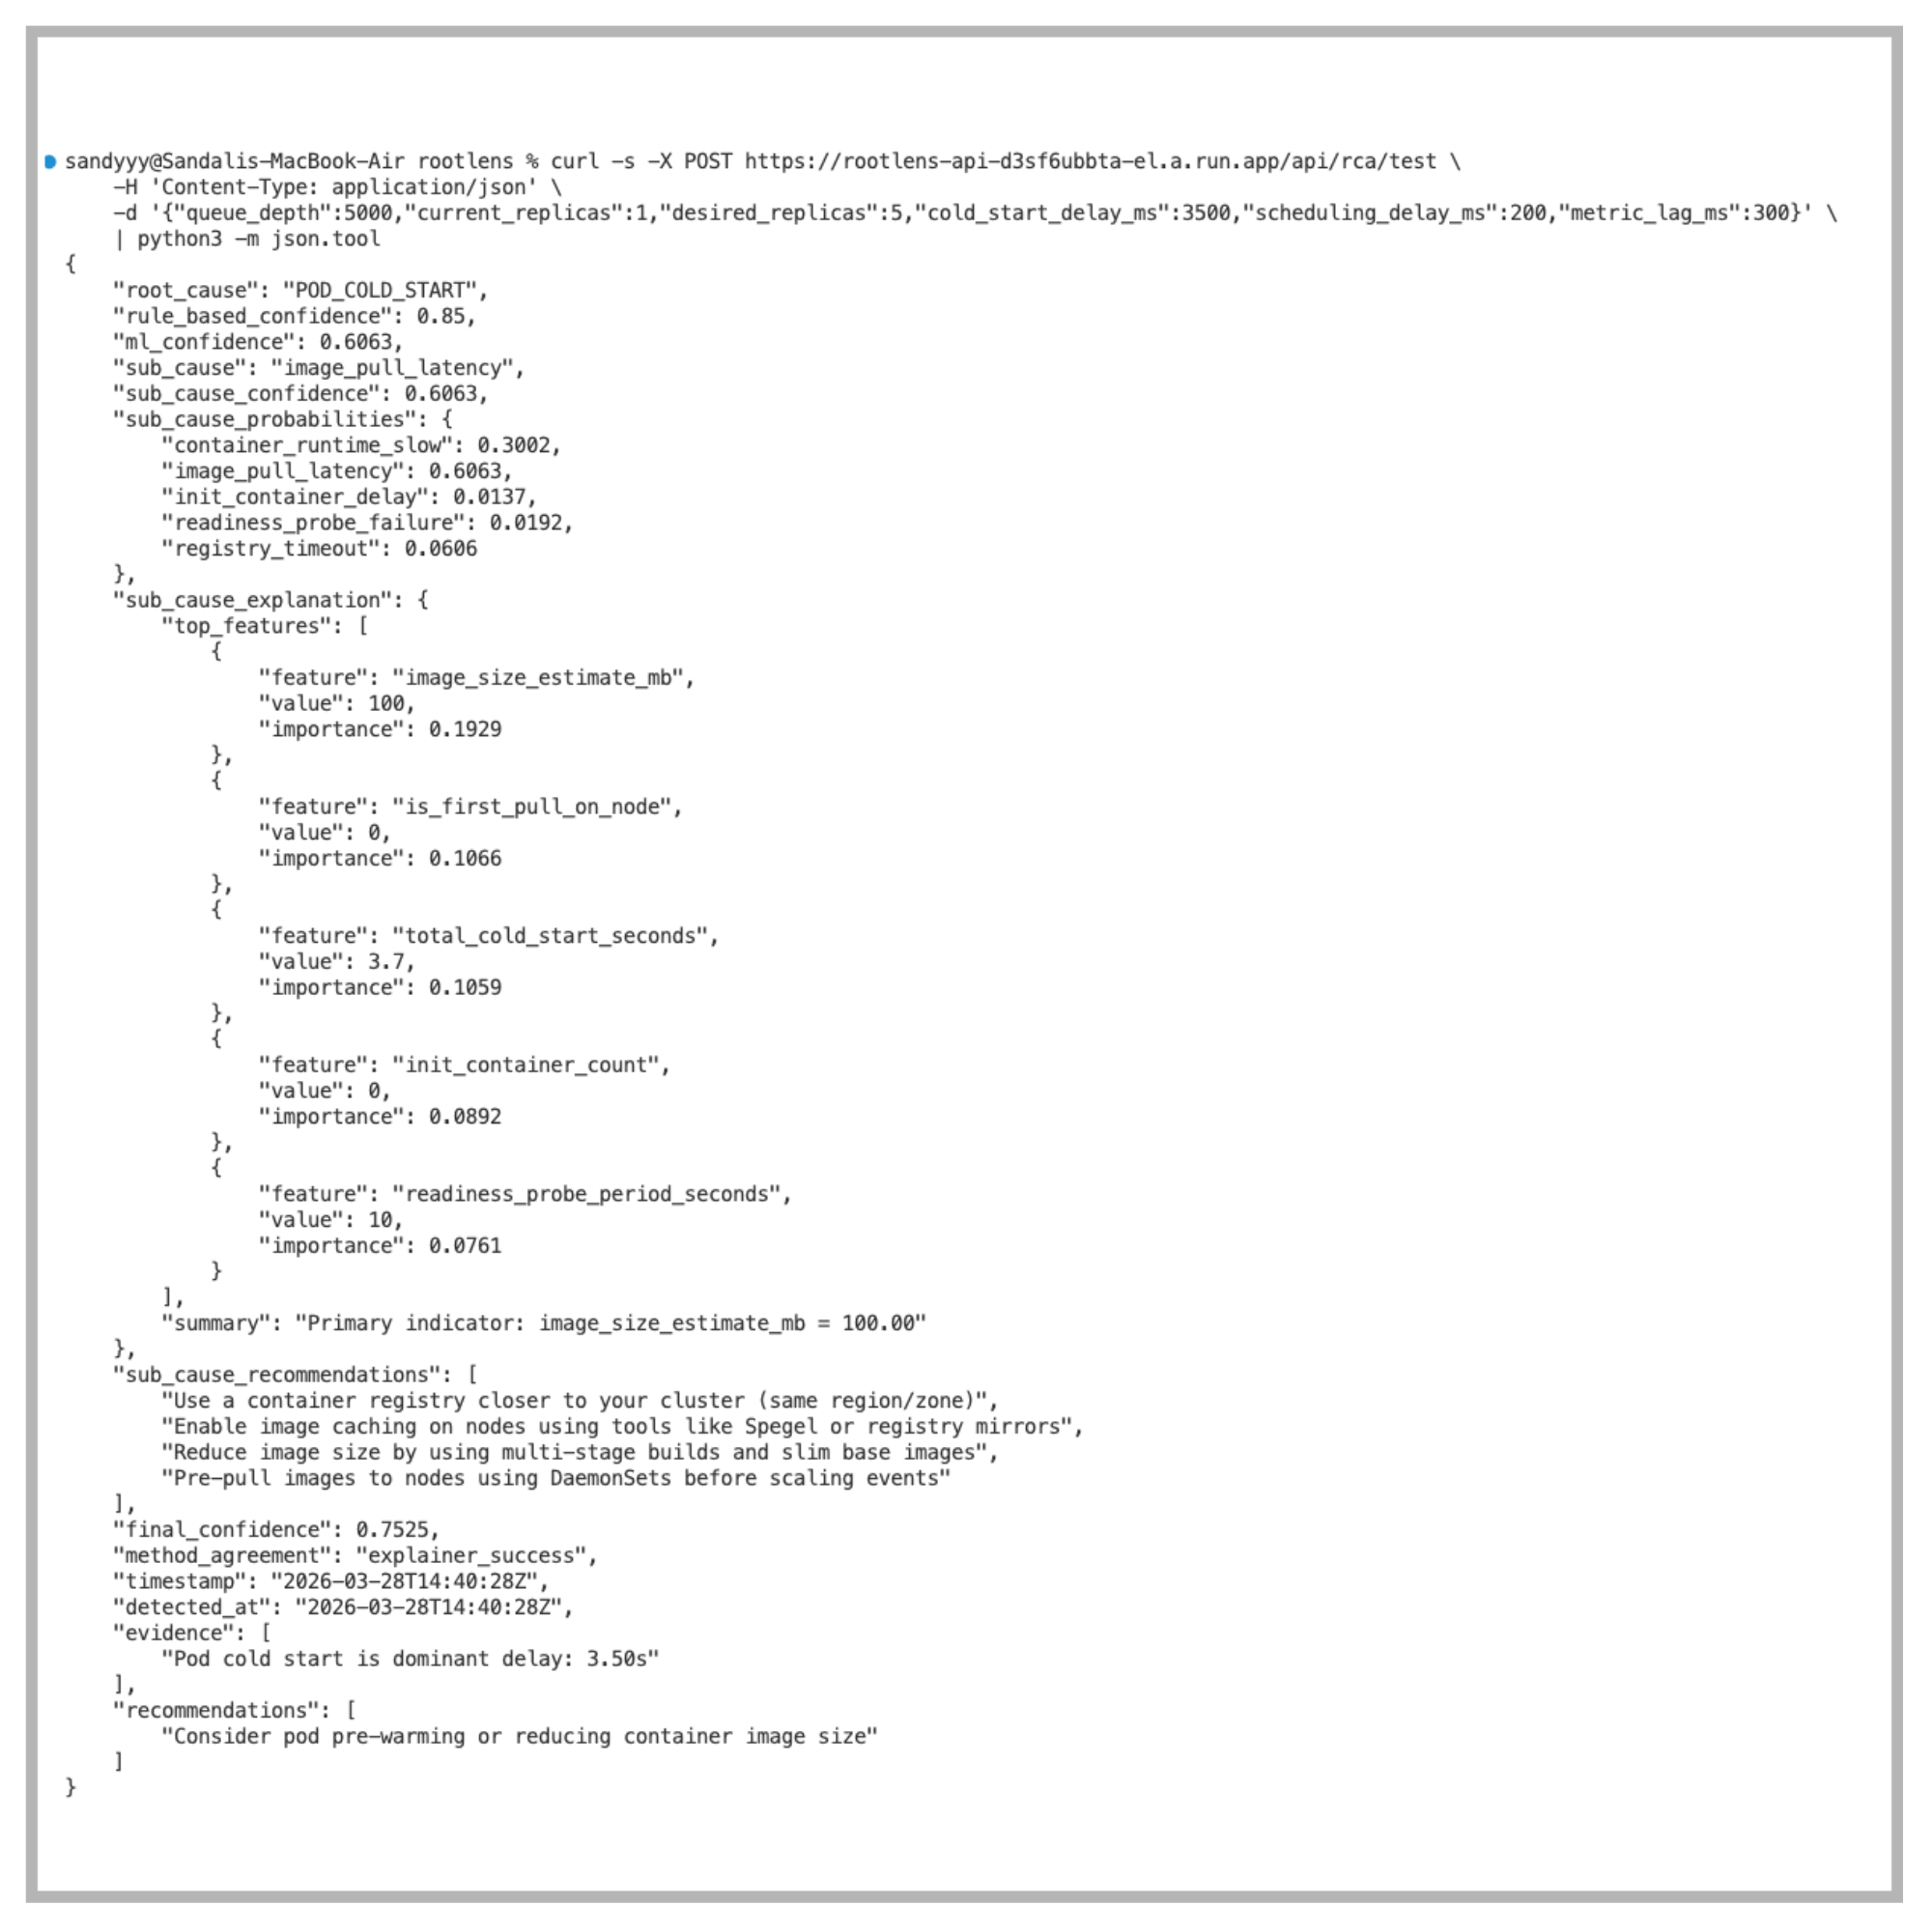
\includegraphics[width=0.66\textwidth]{thesis/assets/cold_start_response.png}
\caption{Sample JSON Response for Cold Start Delays}
\label{fig:api_response_cold}
\end{figure}

\begin{figure}[H]
\centering
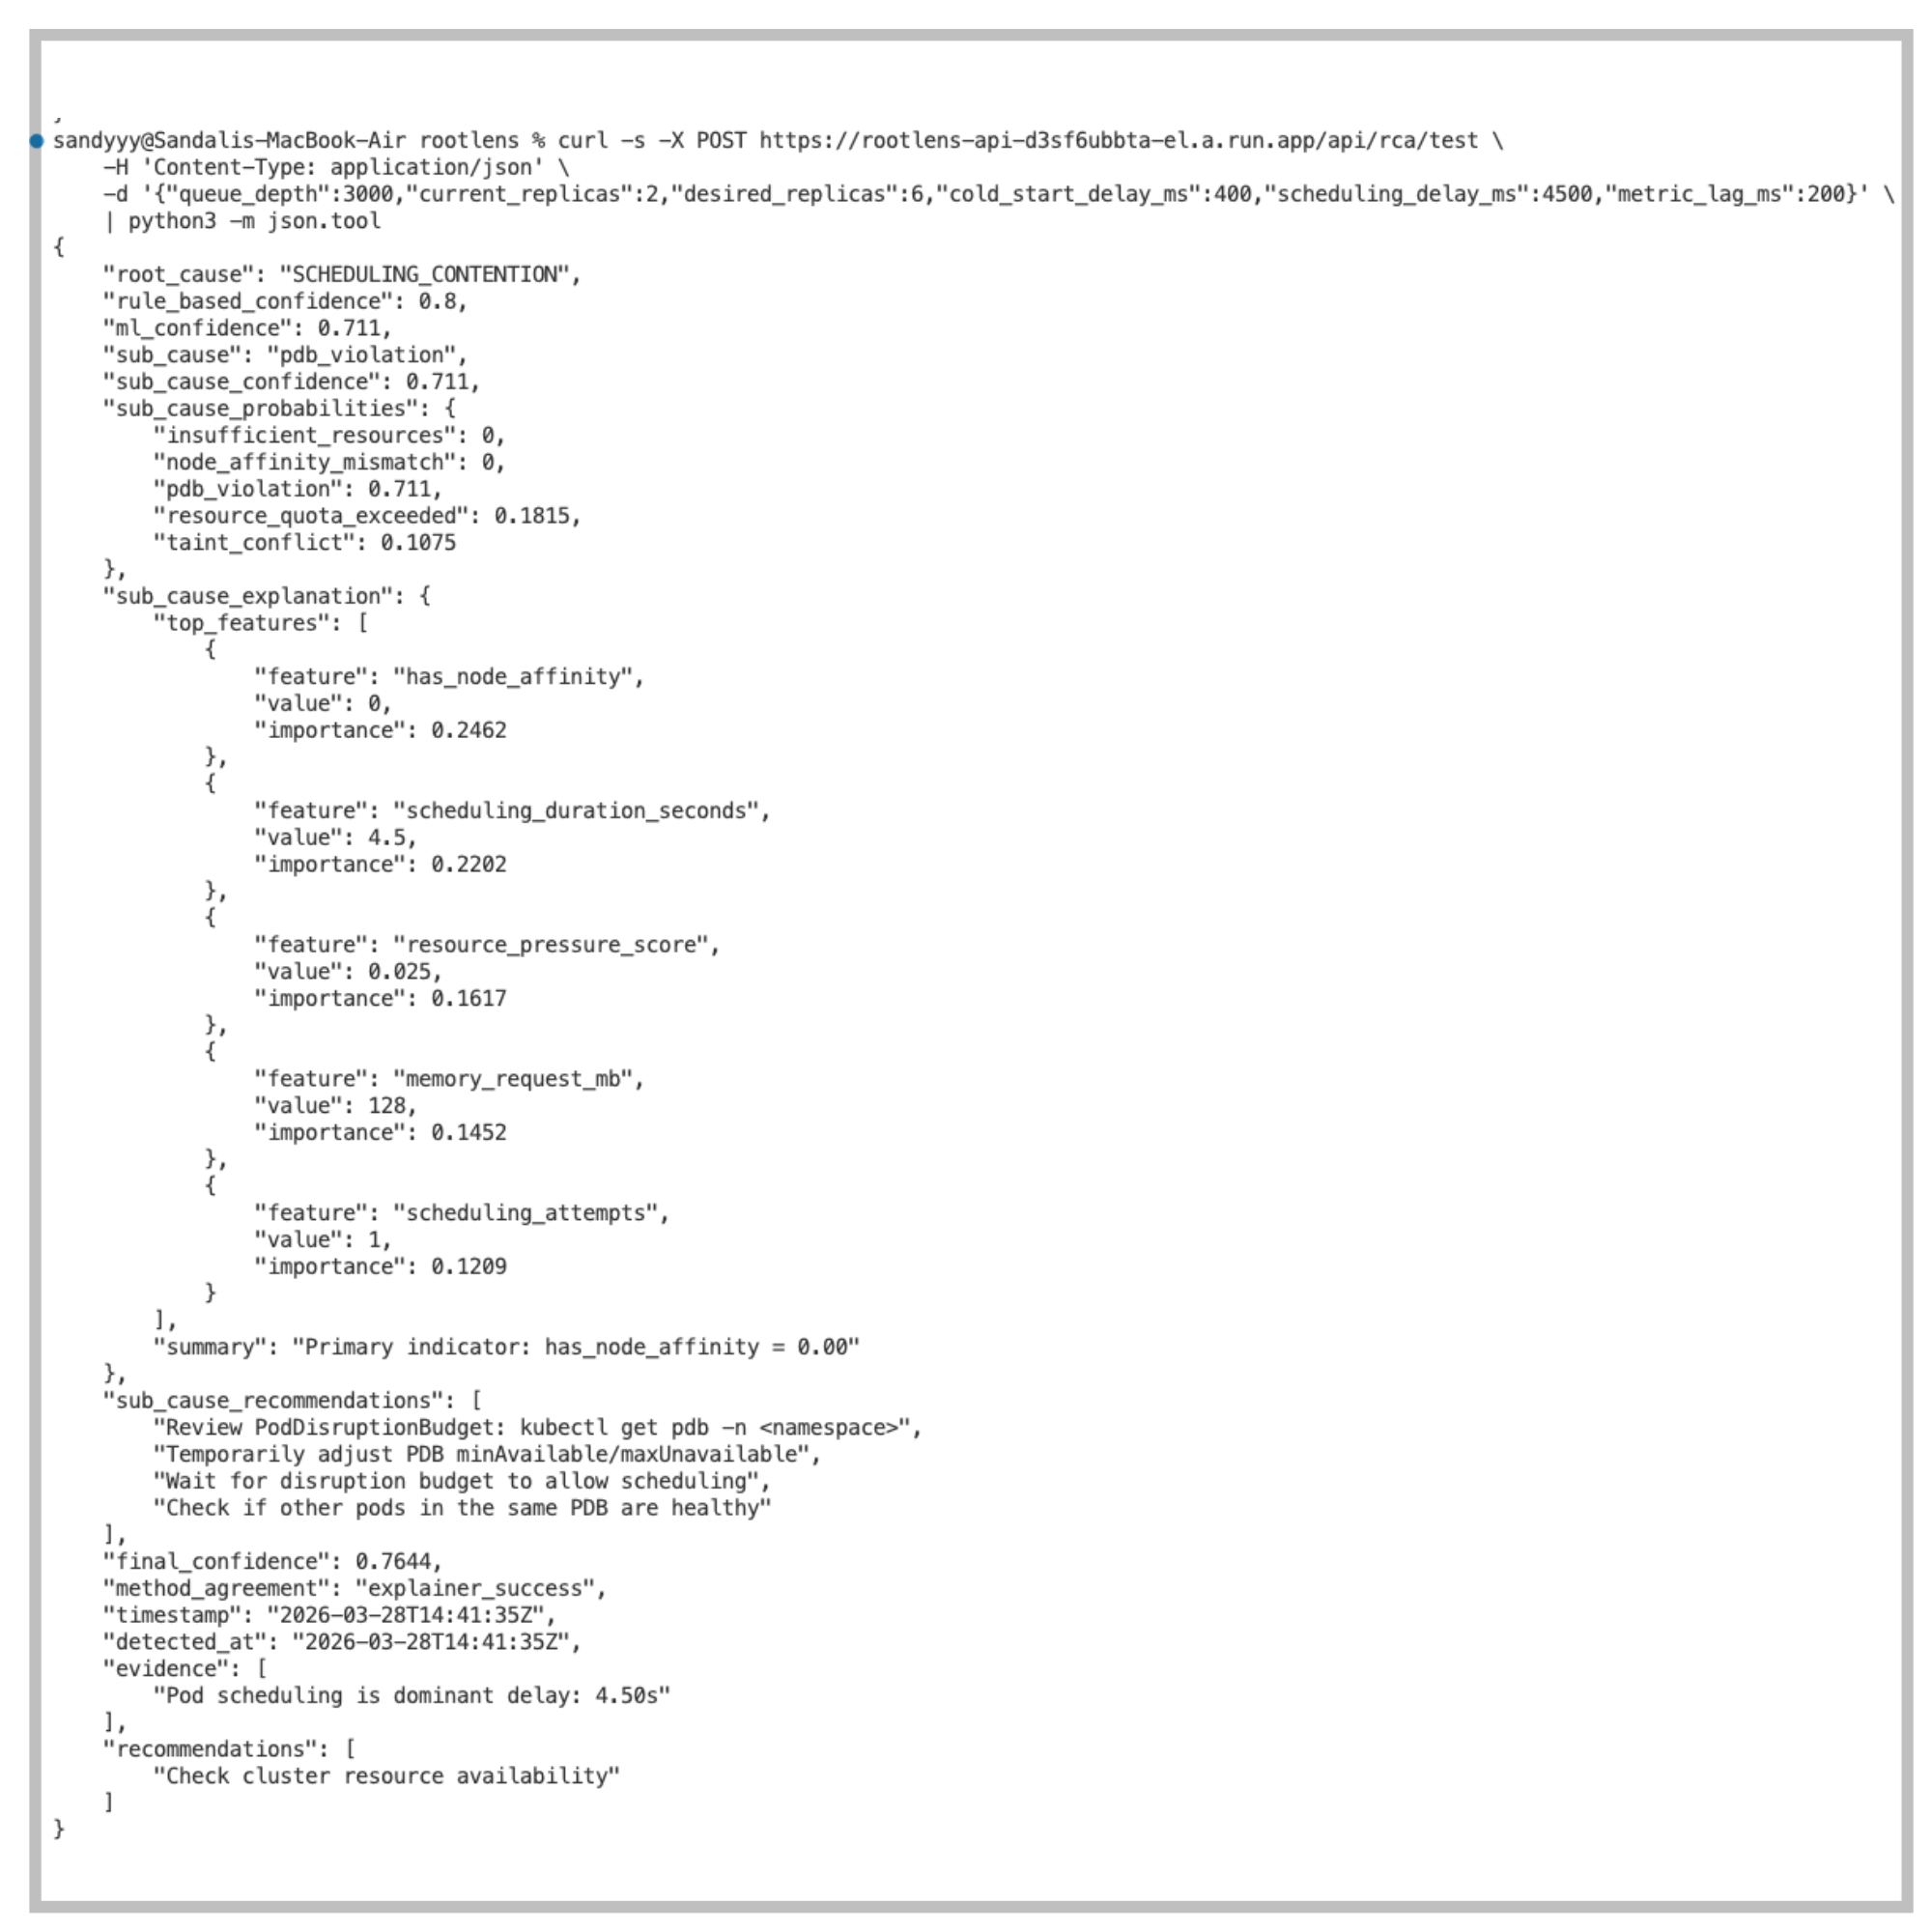
\includegraphics[width=0.66\textwidth]{thesis/assets/scheduling_response.png}
\caption{Sample JSON Response for Scheduling Delays}
\label{fig:api_response_sched}
\end{figure}

\begin{figure}[H]
\centering
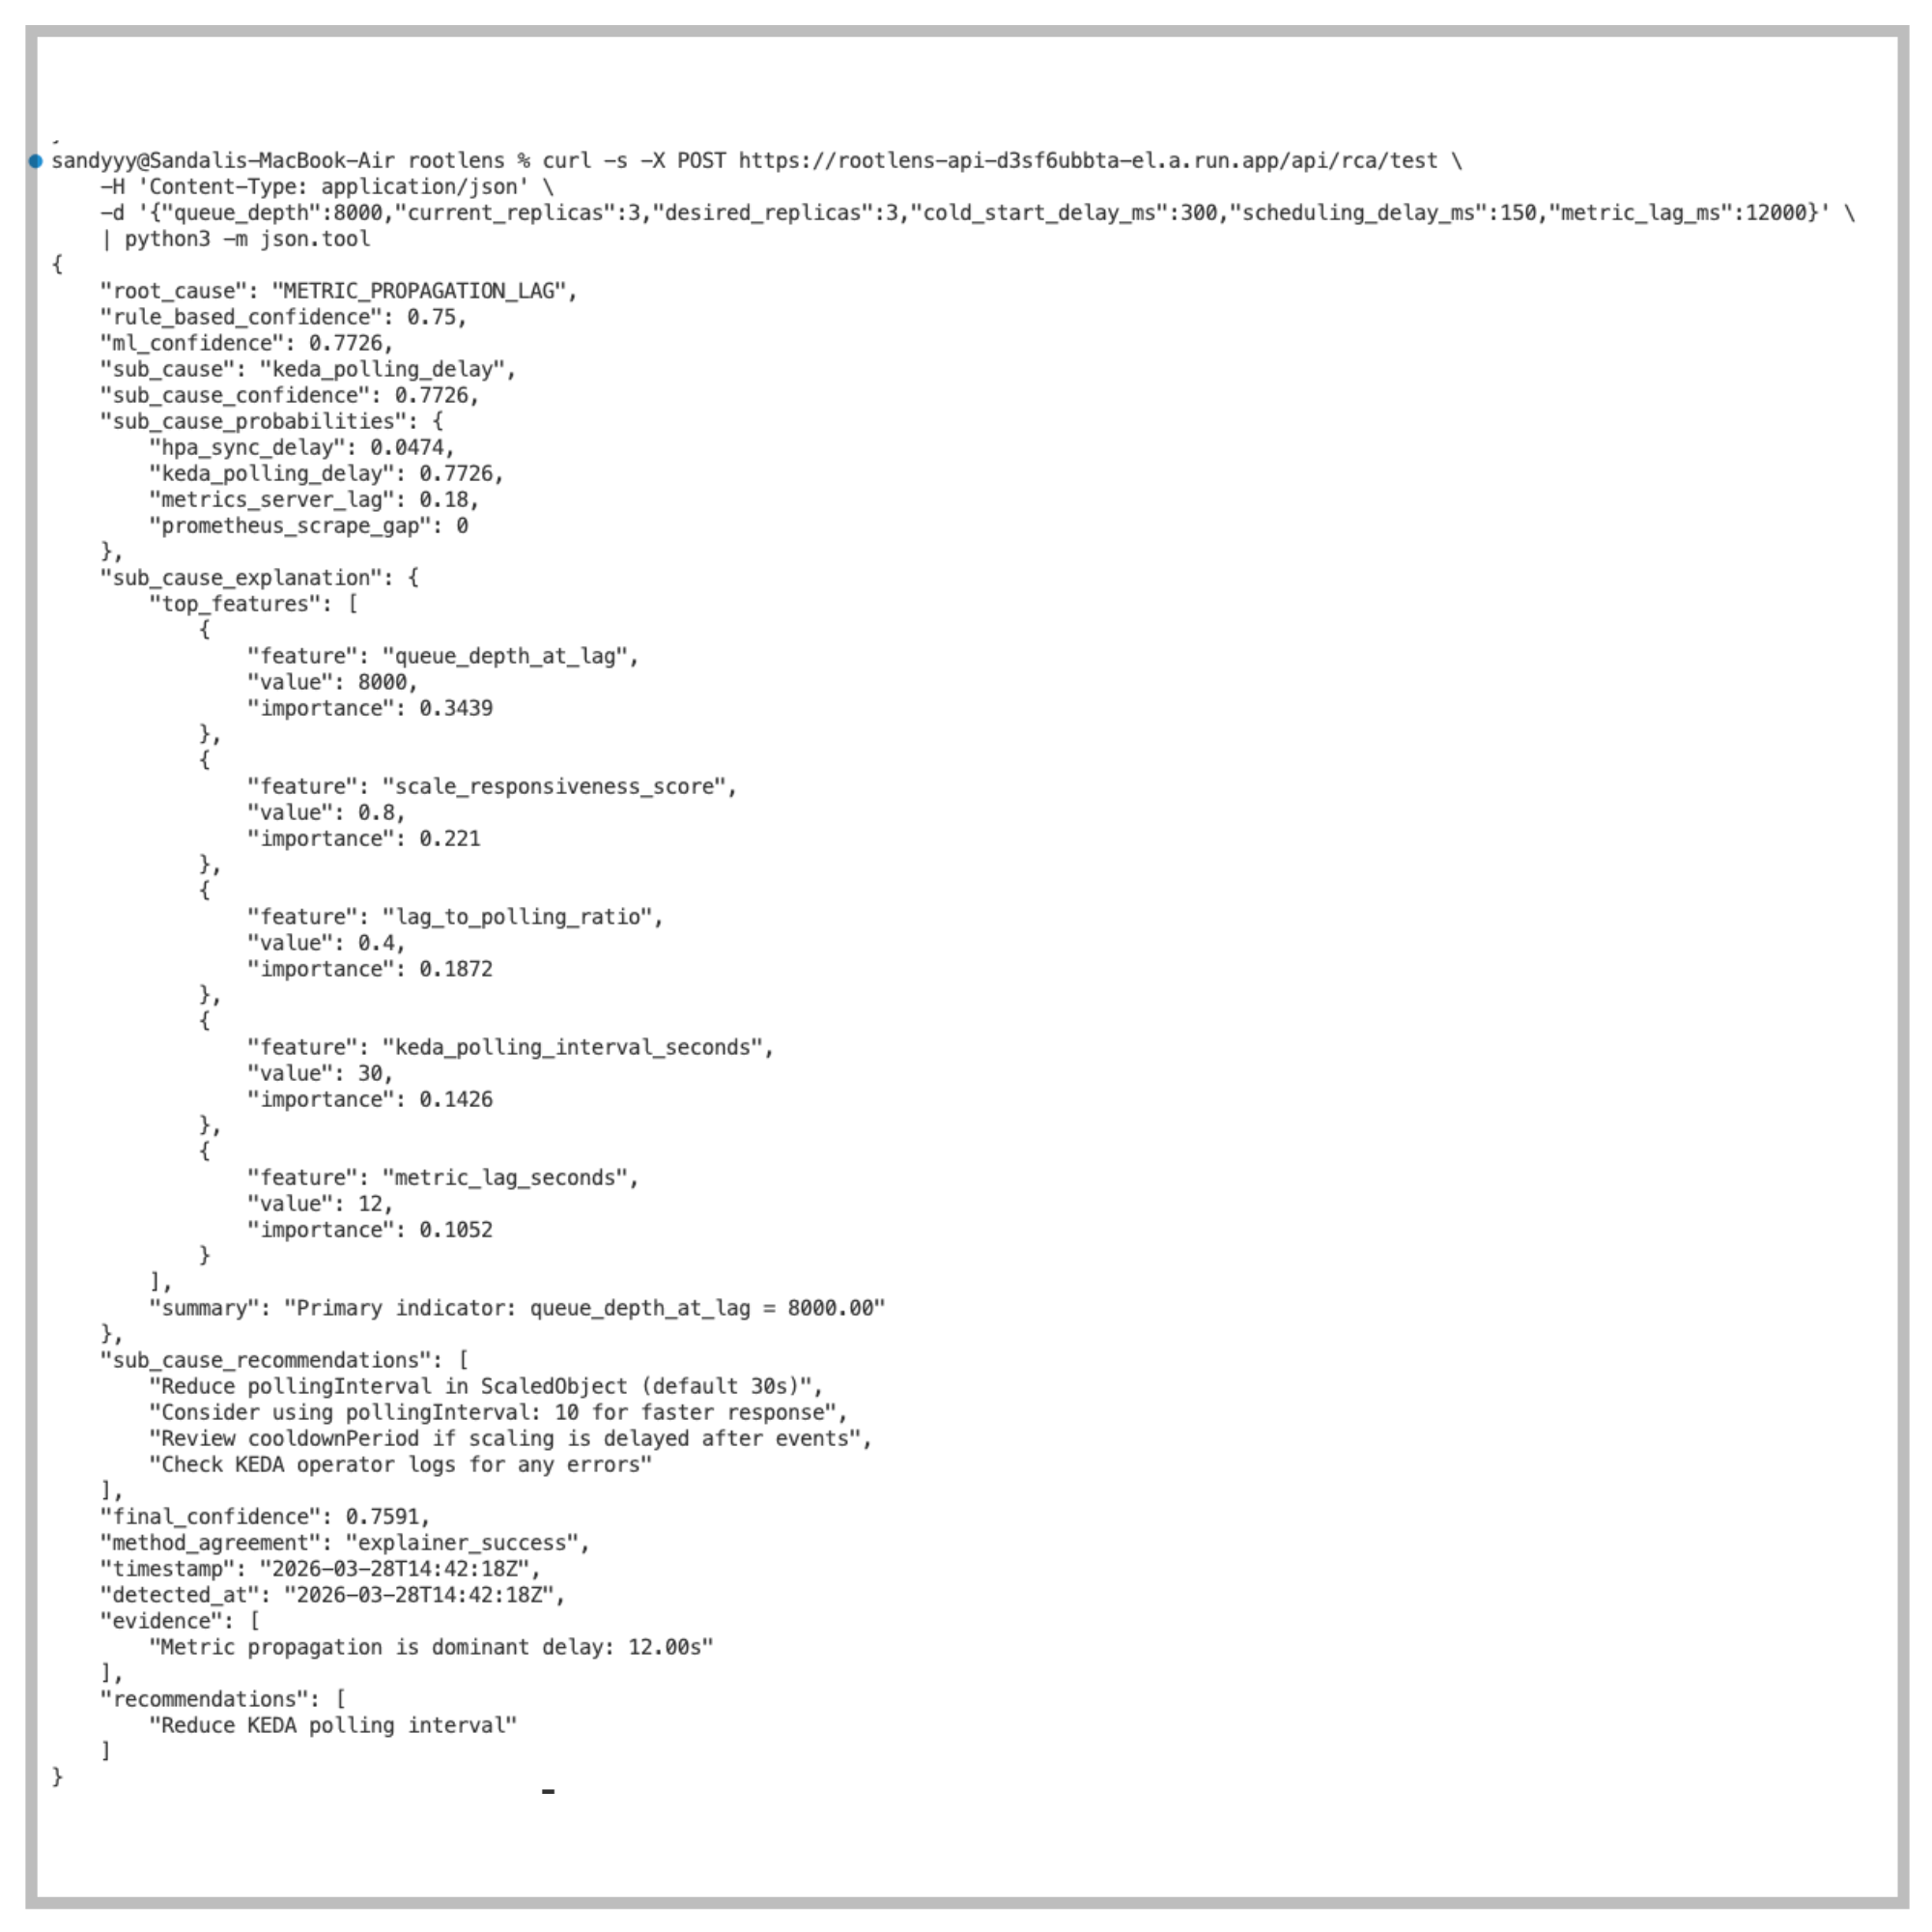
\includegraphics[width=0.66\textwidth]{thesis/assets/metric_propagation_response.png}
\caption{Sample JSON Response for Metric Propagation Delays}
\label{fig:api_response_metric}
\end{figure}

\section{Algorithm Design}
The hybrid RCA process combines rule-based classification with machine learning-based sub-cause prediction, enabling both accurate root cause identification and detailed explanatory insights.

The algorithm operates in two phases: Phase~1 applies deterministic threshold-based rules to classify the root cause category, while Phase~2 routes the feature vector to the appropriate category-specific Random Forest model for sub-cause prediction. The 60/40 weighted confidence combination in line~20 anchors the final score to the rule-based classification while incorporating ML-derived sub-cause certainty.

\section{Design Decisions and Justifications}
The following key design decisions were made during the design phase:

\begin{itemize}
    \item \textbf{Go for the backend:} Go's goroutine-based concurrency model handles thousands of concurrent Kubernetes Watch connections with minimal memory overhead, and its compiled binary produces a 15\,MB container image. Alternative considered: Python (FastAPI), which would have eliminated the service boundary but requires $\sim$200\,MB for a comparable deployment. The trade-off is the added complexity of cross-language communication, mitigated by a well-defined HTTP JSON contract.
    \item \textbf{Python Flask for the ML service:} scikit-learn Random Forest models are natively supported, and Flask provides a lightweight HTTP interface. Separating the ML service allows independent scaling and language-appropriate tooling.
    \item \textbf{60/40 confidence split:} The 60\% rule-based weighting anchors the final score to deterministic classification; the 40\% ML contribution captures sub-cause ambiguity. A 50/50 split produced over-confident scores (mean 0.82) that did not reflect the 86.7\% sub-cause accuracy, while a 70/30 split reduced the ML contribution below useful visibility. The 60/40 split achieved the best alignment between reported confidence and actual classification accuracy.
    \item \textbf{In-memory ring buffer:} Alternative considered: PostgreSQL or SQLite. Persistent storage would enable historical analysis beyond 50 results but would introduce deployment dependencies disproportionate to this proof-of-concept. The ring buffer's O(1) write and O(n) read performance is sufficient for real-time monitoring.
    \item \textbf{Random Forest over alternative ML models:} Provides high accuracy on structured, low-dimensional tabular features with small training sets, natively produces feature importances for explainability, and is robust to feature scale differences. A detailed comparison with SVM, neural networks, and gradient boosted trees is presented in Chapter~3.
    \item \textbf{React dashboard:} A supplementary visualisation component that surfaces RCA results and health status; it does not form part of the core diagnostic pipeline and can be omitted without affecting RCA correctness.
    \item \textbf{Kubernetes Operator:} The kubebuilder-based Operator automates cluster provisioning via a single Custom Resource, providing a repeatable deployment path beyond the Docker Compose prototype.
\end{itemize}

\section{Requirements Traceability}
Table~\ref{tab:design_trace} maps each major design component to the functional and non-functional requirements it satisfies from Chapter~4.

\begin{xltabular}{\textwidth}{|p{3.5cm}|X|p{4cm}|}

\hline
\textbf{Design Component} & \textbf{Purpose} & \textbf{Requirements} \\ \hline
\endfirsthead

\hline
\textbf{Design Component} & \textbf{Purpose} & \textbf{Requirements} \\ \hline
\endhead

Data Collection Module & Real-time K8s event ingestion & FR01, FR02 \\ \hline
Rule-Based RCA Engine & Three-category classification & FR03, NFR02 \\ \hline
ML Explainer Service & Sub-cause prediction & FR04, FR05, NFR03 \\ \hline
60/40 Confidence Model & Calibrated confidence scores & FR06 \\ \hline
Ring Buffer Storage & RCA result history & FR07 \\ \hline
REST API & JSON output for consumers & FR08, FR09, FR10, FR14, NFR01, NFR04 \\ \hline
Graceful Degradation & Rule-based fallback & FR13 \\ \hline
React Dashboard & Visual monitoring interface & FR11, FR12 \\ \hline
Kubernetes Operator & Production deployment & FR15, NFR07 \\ \hline

\caption{Design To Requirements Traceability Matrix}
\label{tab:design_trace}
\end{xltabular}

\section{Chapter Summary}
This chapter presented the complete design of RootLens, from the four-layer architecture through to the detailed design of each component, the API contract, and the in-memory storage design. The rule-based classification equations and ML model specifications define the intelligence layer precisely. Key design decisions were justified with reference to the project constraints and requirements. Chapter 7 describes the implementation of this design in detail.
